\documentclass[tikz,border=4pt]{standalone}
\usepackage{ctex}\usepackage{pgfplots}\pgfplotsset{compat=1.18}
\begin{document}
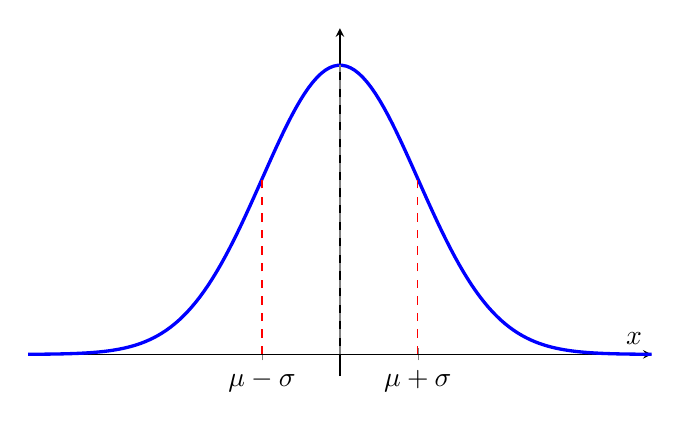
\begin{tikzpicture}
\begin{axis}[axis lines=middle,xlabel={$x$},xmin=-4,xmax=4,ymin=-0.03,ymax=0.45,width=9.5cm,height=6cm,xtick={-1,0,1},xticklabels={$\mu-\sigma$,$\mu$,$\mu+\sigma$},ytick=\empty,samples=150]
\addplot[blue,very thick,domain=-4:4]{exp(-x^2/2)/sqrt(2*pi)};
\draw[dashed,gray](axis cs:0,0)--(axis cs:0,0.399);
\addplot[red,dashed]coordinates{(-1,0)(-1,0.242)};\addplot[red,dashed]coordinates{(1,0)(1,0.242)};
\end{axis}
\end{tikzpicture}
\end{document}
